\documentclass{scrartcl}

\usepackage[utf8]{inputenc}
\usepackage[T1]{fontenc}
\usepackage{lmodern}
\usepackage[ngerman]{babel}
\usepackage{amsmath}
\usepackage{listings}
\usepackage{graphicx}
\usepackage{float}

\usepackage{color} 

%% Commands
\newcommand{\n}{\newline}

\title{User Manual}
\subtitle{King of Jawa}
\author{Jannik Jaberg}
\date{\today}
\begin{document}
\maketitle
\begin{figure}[H]
	
\includegraphics[width=\linewidth]{LOGO.png}
\end{figure}
\tableofcontents
\pagebreak
\section{Starten von King of Jawa}

Damit man spielen kann muss zuerst ein Server gestartet werden. Die erfolgt ganz einfach über de Kommandozeileninput (Das Kommandofenster muss im Ordner gestartet werden in dem sich eure King of Jawa .jar Datei befindet).
\begin{center}
    java -jar “King of Java-0.0.1.jar” server <port>
\end{center}
Angewandt sollte dies so aussehn:
\begin{center}
    java -jar “King of Java-0.0.1.jar” server 22313
\end{center}
Dies sollte diesen Output generieren:\n
\begin{figure}[H]
	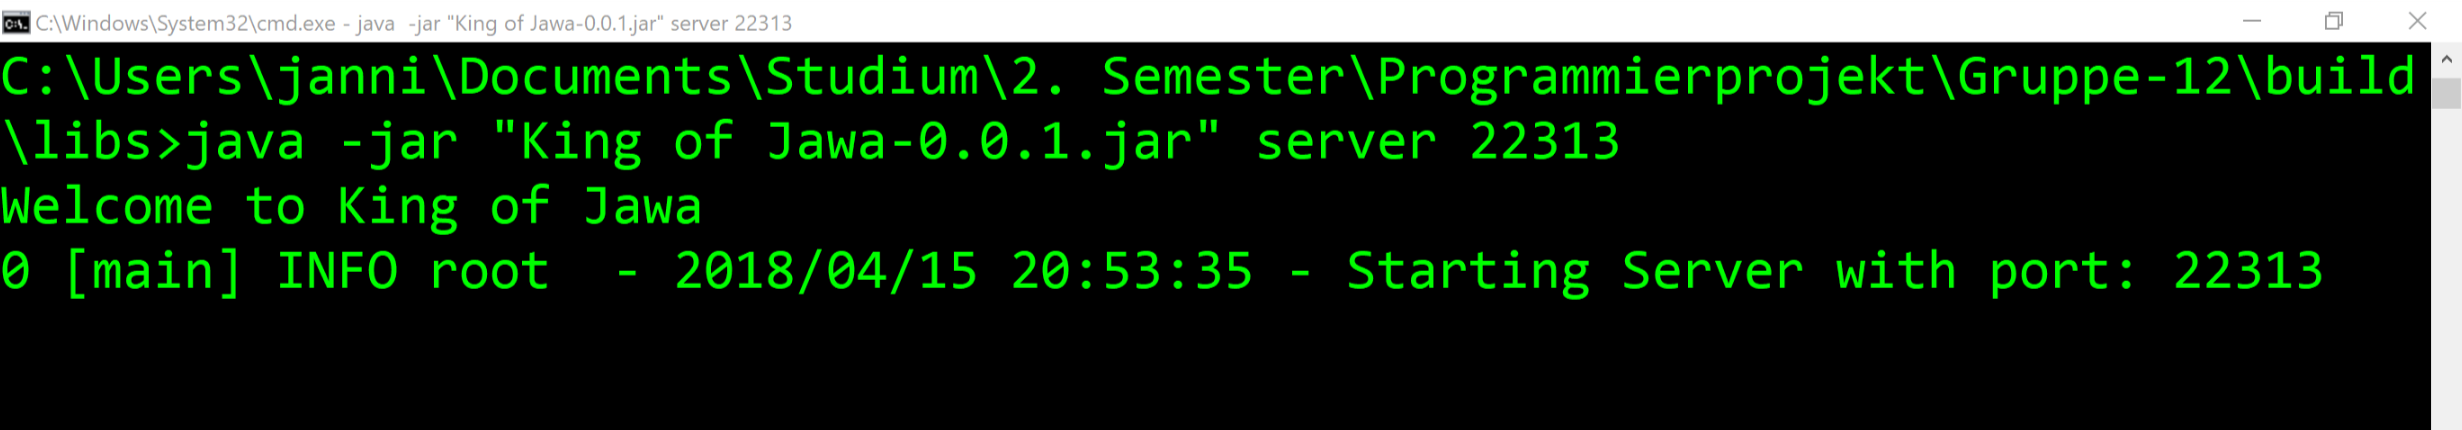
\includegraphics[width=\linewidth]{CMDserver.png}
	\caption{Konsolen-Output Server}
	\label{fig:map1}
\end{figure}
Danach kann von einem neuen CMD Fenster das Spiel gestartet werden mit dem Kommandozeilenbefehl:
\begin{center}
    java -jar “King of Java-0.0.1.jar” client <host>:<port> $[<username>]$ 
\end{center}

Wobei der Username fakultativ ist. Wenn du keinen Username angibst fragt dich das Programm ob du deinen Systemname benützen willst oder nicht, falls du dies nicht willst kannst du einen eigenen Username eingeben. Du kannst danach deinen Username immernoch wechseln über den Command /nick, dazu aber später mehr. \n
Der Host ist die IPv4 Adresse des Hostcomputers (Der Computer auf dem ihr den Server gestartet habt). Demnach sollte der Input etwa so aussehen:
\begin{center}
    java -jar “King of Java-0.0.1.jar” client 192.168.1.122:22313 XxXLaNlOrDXxX
\end{center}
\begin{figure}[H]
	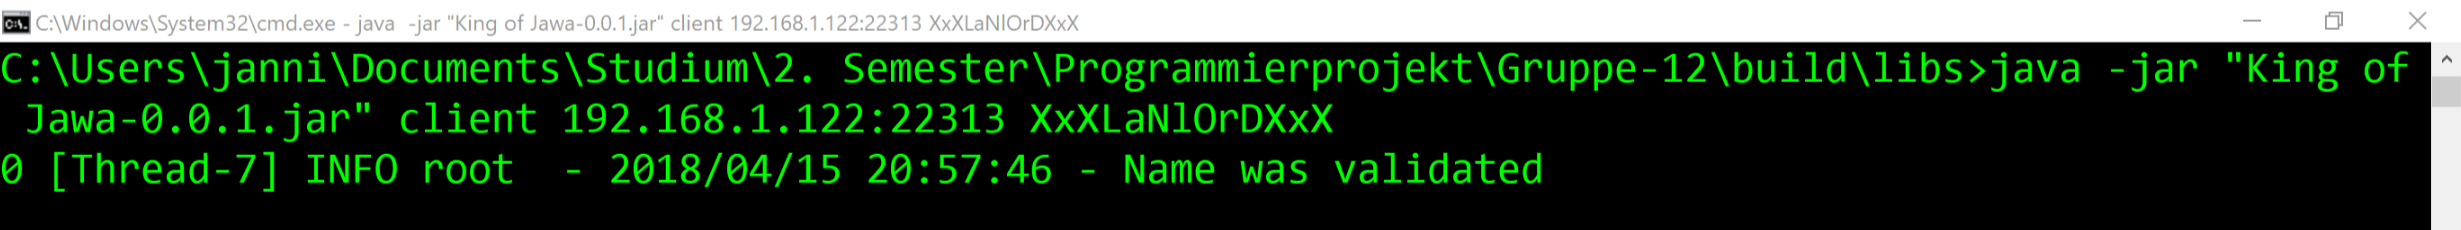
\includegraphics[width=\linewidth]{CMDclient.png}
	\caption{Konsolen-Output Client}
	\label{fig:map1}
\end{figure}
\pagebreak
Wenn alles richtig eingegeben wurde sollte ein Clientfenster geöffnet werden.
\begin{figure}[H]
	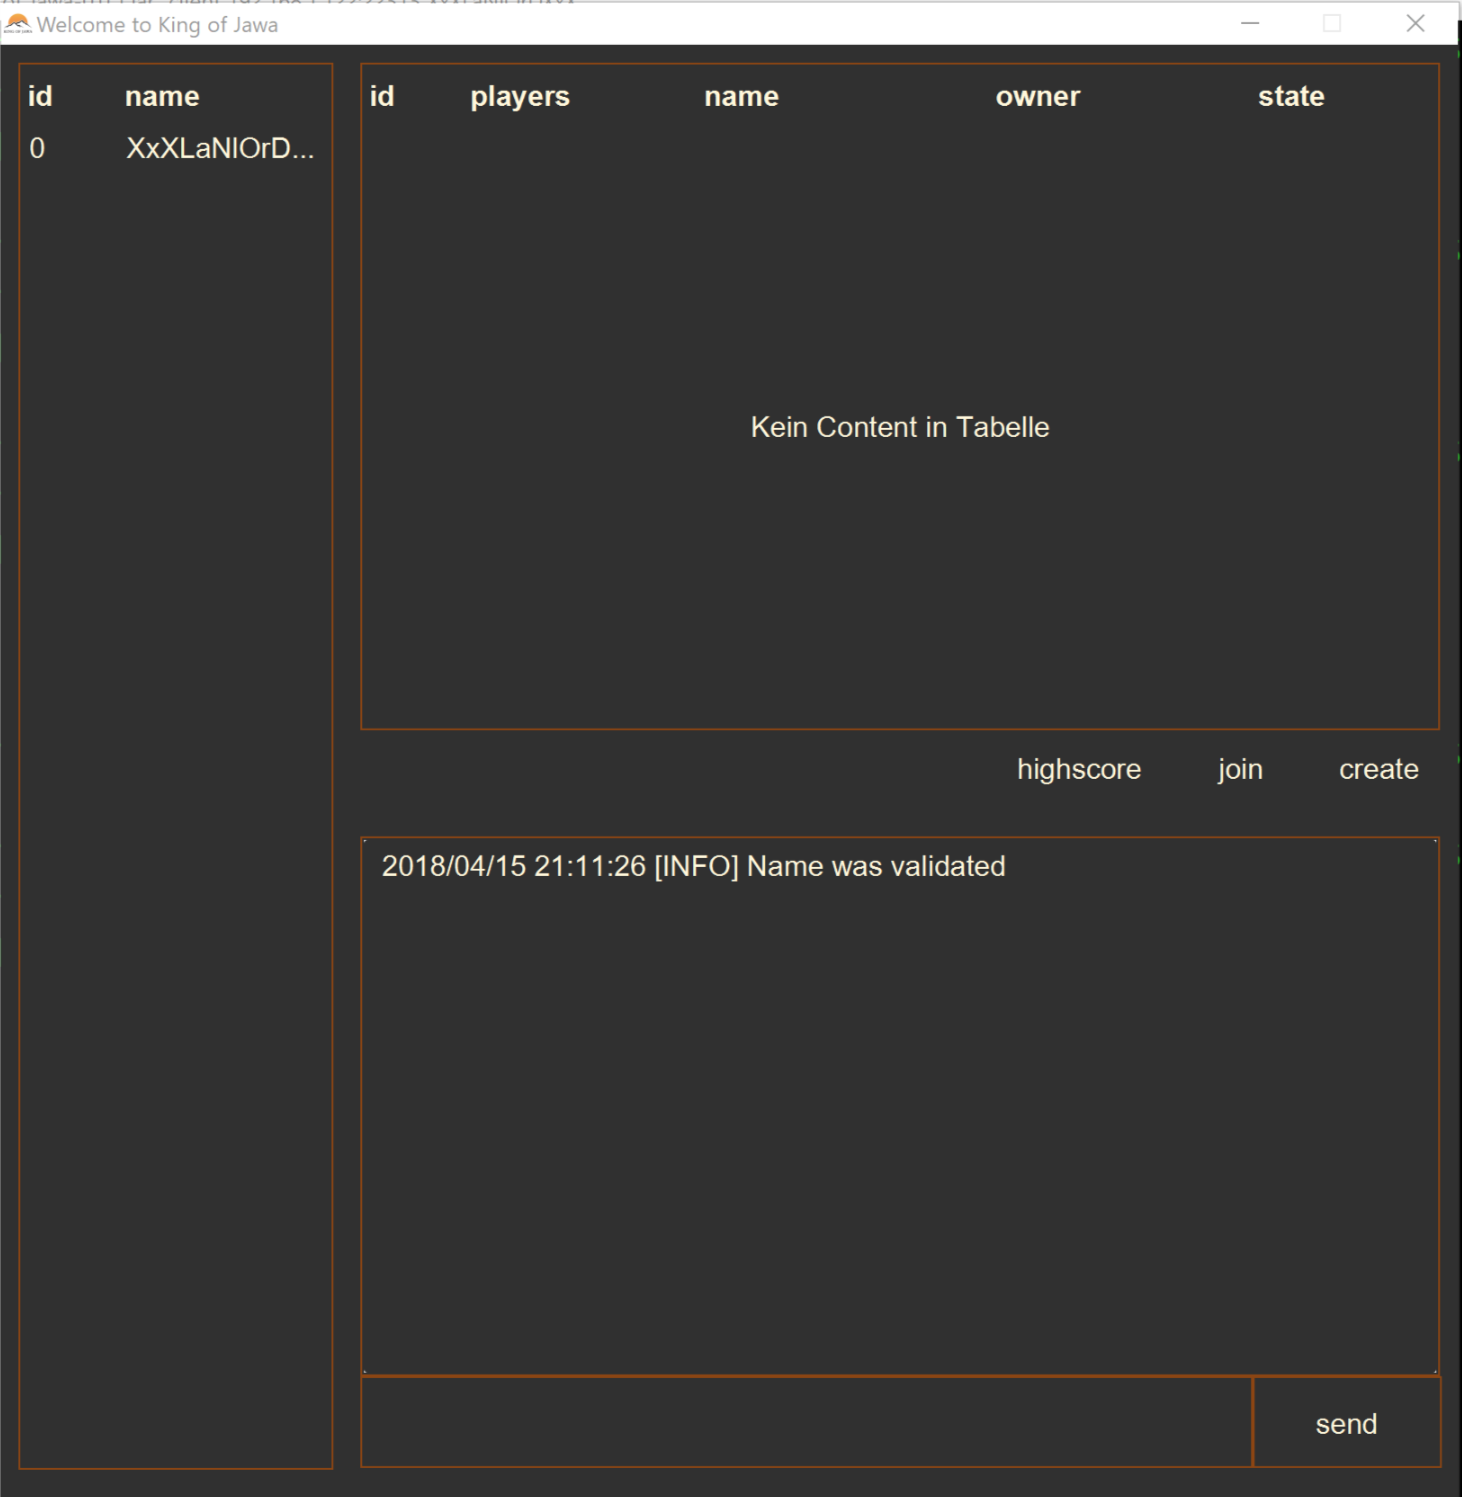
\includegraphics[width=\linewidth]{GUIclient.png}
	\caption{Client-GUI}
	\label{fig:map1}
\end{figure}
Jetzt könnt ihr mit anderen Spielern chatten!

\pagebreak
\section{Commands}
Zurzeit existieren folgende Commands:
\begin{itemize}
    \item /nick <newname>
    \item /whisper <\grqq receipant\grqq> <message>
    \item /ping
    \item /ge
\end{itemize}
  
\begin{center}
    \begin{tabular}{| p{6cm} | p{6cm} |}
        \hline
        \textbf{Anwendung} & \textbf{Nutzen} \\ \hline
        /nick Maximumblyat & ändert deinen Namen   \\ \hline
        /whisper "Habibi" \space GiT GuD & sendet die Nachricht "Git GuD"\space an Habibi  \\ \hline
        /ping & gibt dir deinen Ping an  \\ \hline
        /ge & wenn ihr in einer Lobby oder inGame seid, kann mit /ge in den Global-Chat geschrieben werden. \\ \hline
    \end{tabular}
\end{center}

\begin{figure}[H]
	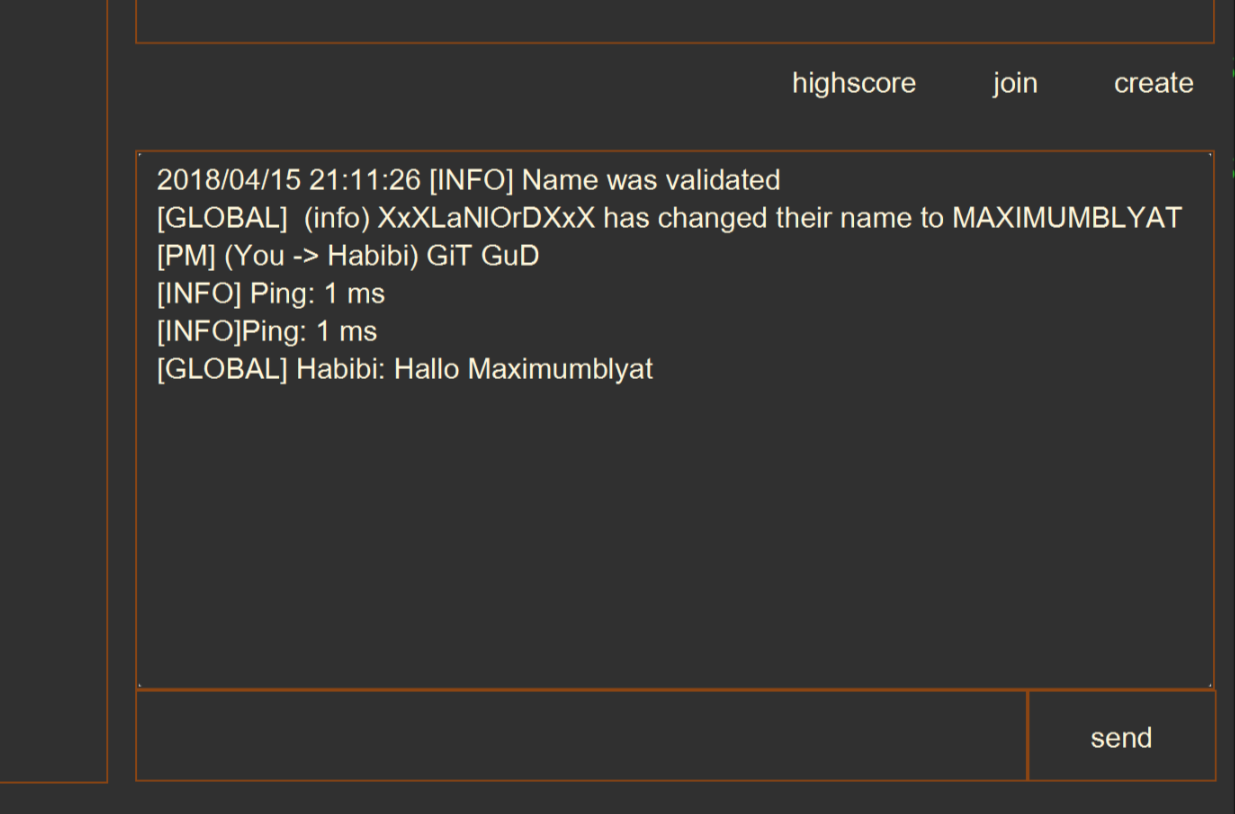
\includegraphics[width=\linewidth]{CMDS.png}
	\caption{Verwendung von CMDs}
	\label{fig:map1}
\end{figure}
\pagebreak
\section{Lobby erstellen und joinen}

Um \textbf{King of Jawa} spielen zu können müsst ihr entweder eine Lobby erstellen und einer bestehenden joinen. Wenn ihr einer Lobby joinen wollt, wählt ihr einfach oben eine Lobby aus und klickt danach join.\n
Um eine Lobby zu erstellen muss man lediglich auf "create" klicken und es öffnet sich ein Lobby-PopUp-Window. Dort könnt ihr die Map aussuchen auf welcher ihr spielen wollt.
\begin{figure}[H]
	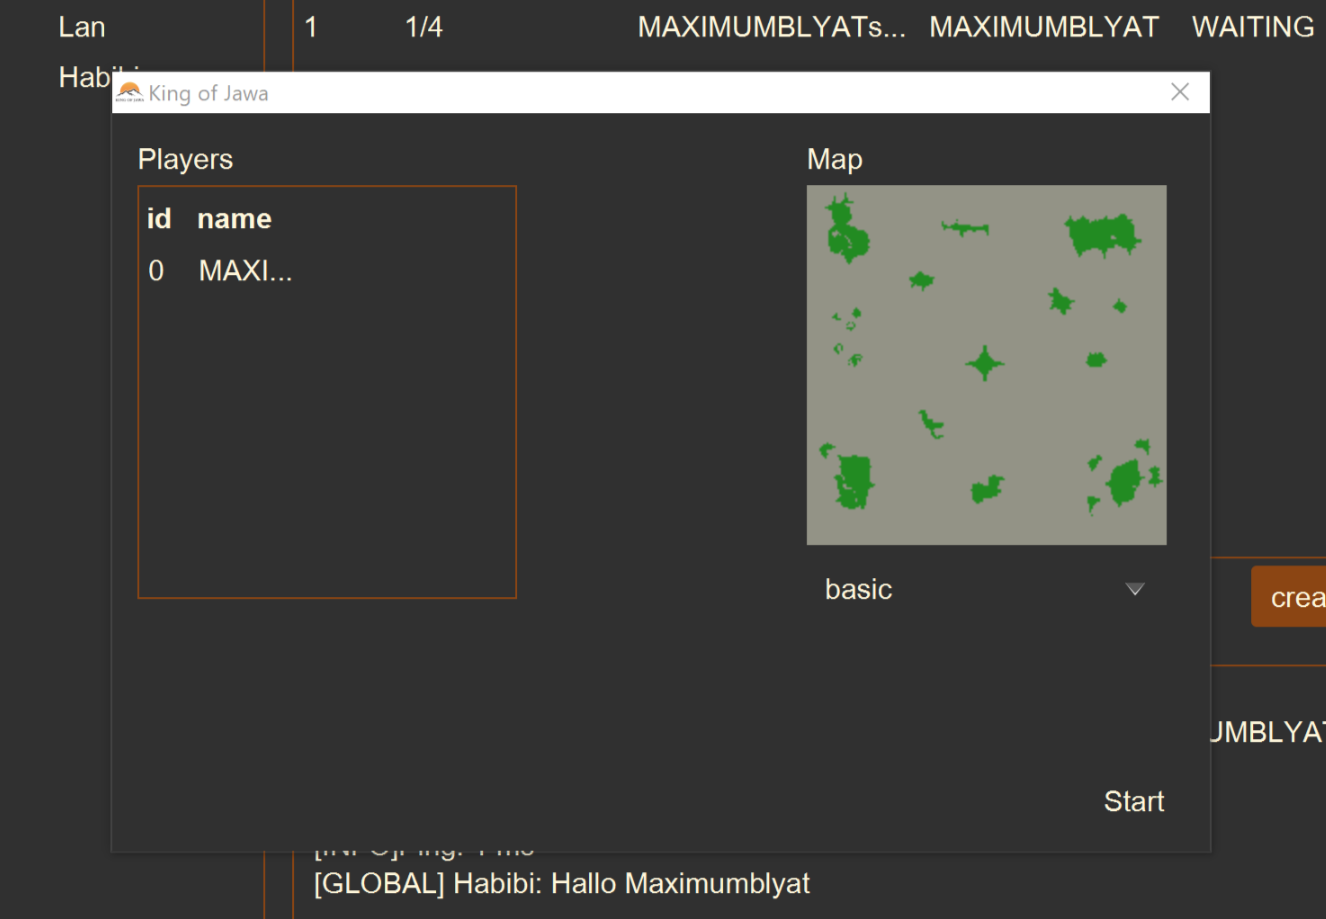
\includegraphics[width=\linewidth]{Lobby.png}
	\caption{Lobby-Window}
	\label{fig:Lobby}
\end{figure}
Wenn all eure Mitspieler begetretten sind und die gewünschte Map ausgewählt ist, klickt einfach auf $"$Start$"$\space und das Spiel geht los.

\pagebreak
\section{Spielregeln}
Direkt nach Spielstart müsst ihr euch für eine Insel entscheiden und sie claimen. Danach gehört diese Insel euch und ihr könnt beginnen eure Metropole aufzubauen.
\subsection{Ressourcen}
Momentan implementierte Resourcen sind: Holz, Stein und Gold. Oben links im Fenster sieht man wie viel Einheiten pro Ressource vorhanden sind. Ganz links in der Ressourcenleiste gibt es nocheinmal eine Steinsymbol, dies steht als platzhalter für die Einwohner.
\subsection{Mini-Map}
Oben rechts im Fenster seht ihr eine Mini-Map bei der in Farbe markiert ist, ob eine Insel frei oder vergeben ist. Mittels klick auf die Mini-Map könnt ihr zum ausgewählten Punkt springen.
\subsection{Gebäude}
Unten links im Fenster ist ein Button (build) mit dem ihr durch die Gebäude wechseln könnt (falls dieser nicht sichtbar ist, einmal Vollbild machen, dann taucht er auf), zur Zeit gibt es die Wood Farm, welche Holz abbaut, und normale Houses, die Habitants generieren und über Steuern Kapital anlegen.
\begin{figure}[H]
	\includegraphics[width=\linewidth]{Game.png}
	\caption{InGame-GUI}
	\label{fig:inGame}
\end{figure}

    

\end{document}